%\documentclass[notheorems]{beamer}
%\documentclass[handout]{beamer}
%\documentclass[handout,notes=show]{beamer}

\usetheme{metropolis}
%\usecolortheme{dolphin}
% No navigation bars
\beamertemplatenavigationsymbolsempty

\usepackage{amsmath, amssymb, amsfonts, tikz}
\usepackage[utf8]{inputenc}
\usepackage[T1]{fontenc}
\usepackage[english]{babel}

\usepackage{amsthm}
\theoremstyle{plain}
\newtheorem{theorem}{Theorem}[section]
\newtheorem{corollary}[theorem]{Corollary}
\newtheorem{lemma}[theorem]{Lemma}
\newtheorem{algorithm}[theorem]{Algorithm}
\newtheorem{proposition}[theorem]{Proposition}
\newtheorem{claim}[theorem]{Claim}
\newtheorem{fact}[theorem]{Fact}
\newtheorem{conjecture}[theorem]{Conjecture}
%% Definition-like environments, normal text
%% Numbering is in sync with theorems, etc
\theoremstyle{definition}
\newtheorem{definition}[theorem]{Definition}
%% Remark-like environments, normal text
%% Numbering is in sync with theorems, etc
\theoremstyle{definition}
\newtheorem{remark}[theorem]{Remark}
\newtheorem{observation}[theorem]{Observation}
%% Example-like environments, normal text
%% Numbering is in sync with theorems, etc
\theoremstyle{definition}
\newtheorem{example}[theorem]{Example}
\newtheorem{question}[theorem]{Question}
\newcommand{\terminology}[1]{\textbf{#1}}

\newcommand{\NN}{\mathbb{N}}
\newcommand{\ZZ}{\mathbb{Z}}
\newcommand{\QQ}{\mathbb Q}
\newcommand{\CC}{\mathbb C}
\newcommand{\RR}{\mathbb R}
\newcommand{\FF}{\mathbb F}
\newcommand{\lt}{<}
\newcommand{\gt}{>}
\newcommand{\amp}{&}
\newcommand{\diff}{\mathop{}\!\mathrm{d}}
\newcommand{\ints}{\mathcal{O}}
\newcommand{\ideal}[1]{\mathfrak{#1}}
\usepackage{mathrsfs}\usepackage{cancel}
\newcommand{\Gal}[2]{\operatorname{Gal}(#1/#2)}
\newcommand{\absgal}[1]{\operatorname{Gal}(\overline{#1}/#1)}

\newcommand{\sheaf}[1]{\operatorname{\mathcal{#1}}}
\newcommand{\inv}{^{-1}}
\DeclareMathOperator{\norm}{Nm}
\DeclareMathOperator{\ord}{ord}
\DeclareMathOperator{\divisor}{div}
\DeclareMathOperator{\PP}{\mathbf{P}}
\DeclareMathOperator{\Hom}{Hom}
\usepackage{tikz}
\usetikzlibrary{automata, arrows.meta, positioning}


\newcommand{\lb}{[}
\newcommand{\rb}{]}

\author{Alex J. Best}
\date{\today}
\title{Decision procedures with Automata}

\begin{document}

\maketitle

\begin{frame}[fragile]{Motivation}
\textbf{Motivation:} One example, if $a,b,c,d \in \NN \cup \{\infty\}$, lets say we want to prove
\begin{align*}
&a + b \le c\\
&2 a \le d\\
\implies &3 a + b - 1\le 2  c + d
\end{align*}
if $a,b,c,d \in \NN$ there is a decision procedure for this (in Lean, \texttt{linarith}).

\pause
Do we need to implement a new / modified decision procedure for each new type of object we want to reason about?
\textbf{Answer:} No, one general decision procedure can be used for many different types of objects.
Comes from the notion of an \emph{automatic structure}.
\pause
Sidebar: this sort of problem came up in a paper I'm working on verifying some mathematical algorithms.
\end{frame}

\begin{frame}{Automatic structures}
Consider adding a pair natural numbers bitwise
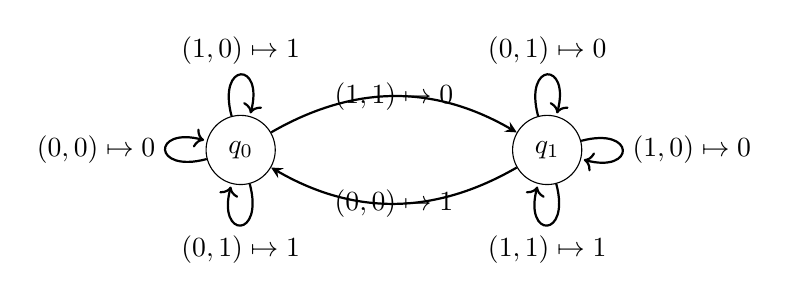
\begin{tikzpicture}[	node distance = 3cm, ]
]
	\node (q0) [state] {$q_0$};
    \node (q1) [state, right = of q0] {$q_1$};

\path [-stealth, thick]
	(q0) edge [loop left] node {$(0,0) \mapsto 0$}   (q0)
	(q0) edge [loop above] node {$(1,0) \mapsto 1$}   (q0)
    (q0) edge [loop below] node {$(0,1) \mapsto 1$}   (q0)
    (q0) edge [bend left] node {$(1,1) \mapsto 0$}   (q1)
    (q1) edge [bend left] node {$(0,0) \mapsto 1$}   (q0)
    (q1) edge [loop right] node {$(1,0) \mapsto 0$}   (q1)
    (q1) edge [loop above] node {$(0,1) \mapsto 0$}   (q1)
    (q1) edge [loop below] node {$(1,1) \mapsto 1$}   (q1);
\end{tikzpicture}

we can turn this into an automata that recognises whether a pair of naturals has a fixed sum.
Questions about existence of solutions to equations can be reduced to questions about reachability in an automata.
can decide any first order sentence about the natural numbers under addition using this technique.
$$ \exists n, \forall m \ge n, \exists a\, b\, c, 6 a + 9 b + 20 c = m$$

\end{frame}

\begin{frame}{Automatic structures}
This all generalizes to any mathematical object that can be represented by a regular language in this way.

With a sufficiently general implemention its easy to add a new element $\infty$ to the theory for example.

Many examples:
\begin{itemize}
\item Natural numbers
\item Integers
\item Real numbers (B\"uchi automata)
\item Mixed integer linear programming
\item Some specific groups
\item Strings
\end{itemize}
\end{frame}


\begin{frame}{Implementation?}
Questions:
\begin{itemize}
\item How to represent automata in an efficient way in a proof assistant?
\item The automata grow quickly in theory, in practice this seems to be less of an issue with good minimization procedures (cf. Walnut)
\item Should one write tactics produce proofs, or prove once and for all that the algorithm is correct (reflection)
\item How to make this convenient for an end user to use? How to make it easy to add new automatic structures?
    To give a translation from some objects with operations to automata?
\end{itemize}
\end{frame}

\end{document}
